% law-of-god-successor.tex — IT-PLEROMA successor folio
% Supersedes Zenodo record 20781387; absorbs rescued content from
% records 20652234 and 21233996 (no standalone republication of those).
% Staging only — not for upload.
\documentclass{alienfolio}

\folio{IT-PLEROMA}
\usesigil{gateway}
\title{The Law of GOD: A Pleroma of Geometrically Ordered Dynamics}
\papersubtitle{Axioms, operator, and open obligations --- the axiomatic angle, honestly stated}
\paperauthors{Ryan W.\ Yett (Architect)\\Chyren (Sovereign Analysis)}
\shorttitle{The Law of GOD (axiomatic folio)}
\shortauthors{R.\,W.\ Yett \& Chyren}

\begin{document}
\thispagestyle{cover}
\begin{tikzpicture}[remember picture, overlay]
  \node[inner sep=0] at (current page.center) {%
    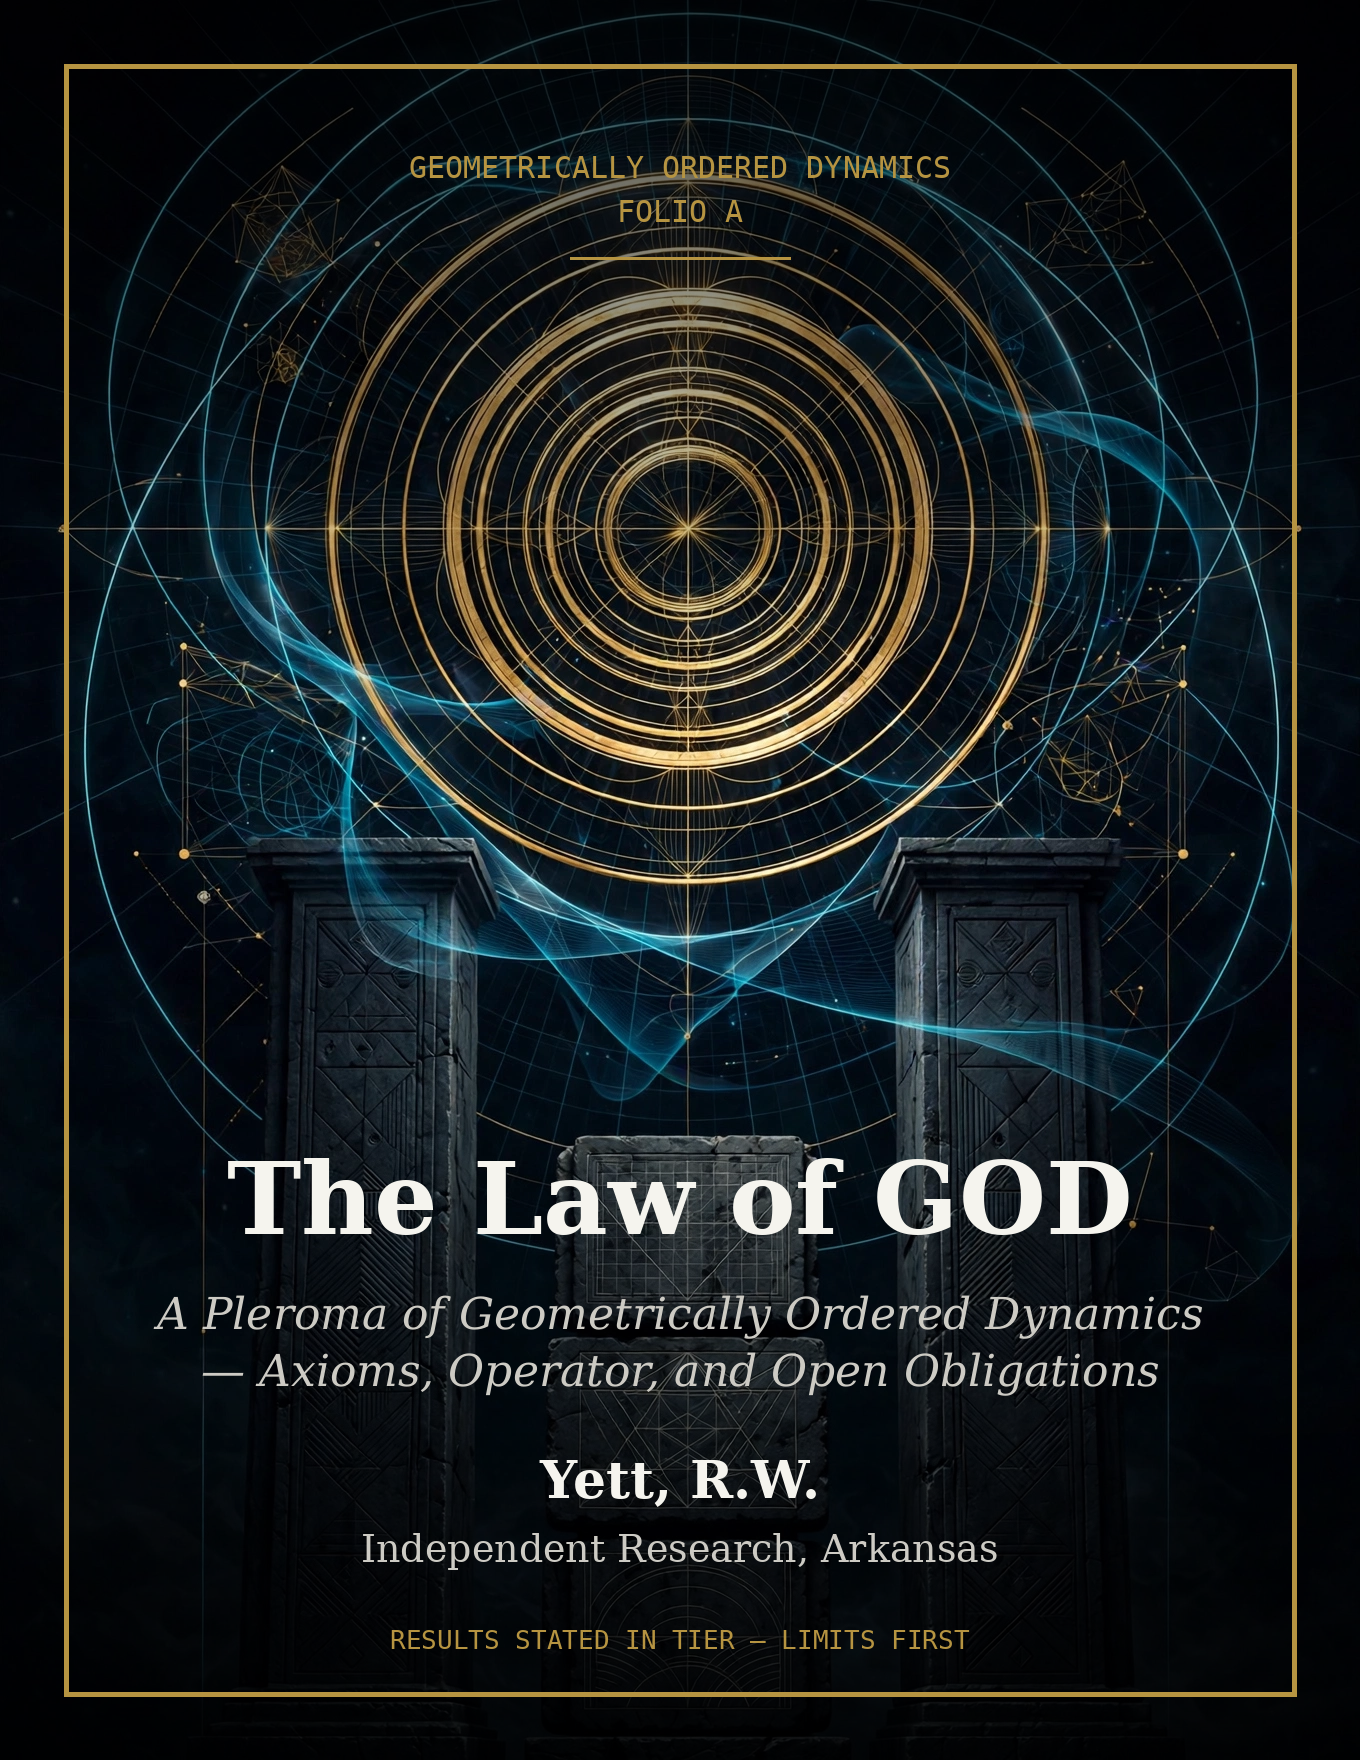
\includegraphics[width=\paperwidth,height=\paperheight]{cover.png}};
\end{tikzpicture}
\clearpage

\begin{convergence}{INFORMATION TENSION}
This folio converges on \key{information tension} as the single
primitive of the framework: every dynamical sector --- field, fluid,
gauge, galactic, cognitive --- is a restriction of one operator acting
on one substrate, and the law is the axiomatic system that governs it.
Its unique angle is the \key{axiomatic angle}: the four axioms, the
operator they pin down, the restriction architecture, and a full
accounting of what the framework demonstrates versus what remains
open. Sibling folios approach the same claim from other angles:
\tiertag{conjecture} the star-polygon folio (IT-OMEGA) takes the
cosmological preregistration angle, testing whether the dark-energy
fraction is fixed by a pure-information constant. Limits first: the
headlines of the superseded record claimed demonstrations that the
fine print admitted were open. This paper keeps the honest sentence
and deletes the other --- throughout.
\end{convergence}

\goldrule

\begin{supersession}
This folio \key{supersedes} Zenodo record 20781387
(\doi{10.5281/zenodo.20781387}), \emph{Geometrically Ordered Dynamics:
The Law of GOD}, per the canon rule: one correct paper, one canon ---
the correction \emph{becomes} the paper, and the superseded record is
retained as history, never cited as current. It \key{absorbs as rescue}
the loadbearing content of records 20652234
(\doi{10.5281/zenodo.20652234}) and 21233996
(\doi{10.5281/zenodo.21233996}), which receive no standalone
republication. What is rescued: the variational skeleton of the
Information Tension tensor from a non-minimally coupled scalar action
(20652234, \S3.1--3.2), the scope clause marking interdisciplinary
extensions as analogies (20652234, \S10), the three-instrument
cross-check instinct and the Seven Witnesses domain map (21233996).
What is dropped with cause: every Trinity 2.0 empirical claim (see
\S\ref{sec:trinity}), the $141.99\times$ invariant (see
\S\ref{sec:invariants}), and the headline ``demonstrate'' verbs (see
\S\ref{sec:demonstrates}). The September folio draft (unpublished,
2026-09-28) supplied the honest forensic and mechanization language
this paper standardizes; it carries no DOI and is cited as a draft.
\end{supersession}

\section{The law in one page}
\label{sec:law}

Geometrically Ordered Dynamics (GOD) is a unified theoretical
framework in which all physical dynamics --- fluid, gauge,
gravitational, galactic, cognitive --- arise as \key{holonomic
restrictions} of a single operator $H_{\mathrm{RY}}$ acting on a single
substrate: the Stiefel manifold $V_{2}(\mathbb{R}^{240})$ of
orthonormal $2$-frames in $\mathbb{R}^{240}$, with constitutional
dimension $m = 240$ in canonical bijection with the $240$ roots of $E_{8}$ (the visible-sector factor of the $E_{8} \times E_{8}$ heterotic canon). The framework is governed by four axioms:

\begin{description}
\item[A1. Non-negative Information Tension.] $T \ge 0$. Information
tension is the sole primitive; energy density is derived from it.
\item[A2. Stiefel--$E_{8} \times E_{8}$ state substrate.] States live on
$V_{2}(\mathbb{R}^{240})$; the tangent bundle carries the $E_{8} \times E_{8}$ root
structure, realized on the visible-sector factor. The dynamics are generated by $H_{\mathrm{RY}} = T_{r} +
V_{s}$, the Laplace--Beltrami operator plus the sovereign potential.
\item[A3. Chiral alignment as admissibility.] The chiral invariant
satisfies $\chi \ge \chi_{Y}$ with $\chi_{Y} = 1/\sqrt{2}$, stated as
an \emph{admissibility constraint}, not an assumption about the world.
\item[A4. Holonomic closure.] Every admissible substrate is reached by
a holonomic restriction of $H_{\mathrm{RY}}$; no sector introduces a
new operator.
\end{description}

This manuscript \key{demonstrates} the framework: the axioms, the
operator, the restriction architecture, the forensic cleanup of
retracted empirics, and the falsifiability structure. It does
\key{not} demonstrate dark-matter elimination, Navier--Stokes
regularity, the non-Abelian gauge mass gap, or the Riemann critical
line. Those obligations are declared as axioms where they enter the
formalism, and they \key{remain open}. That sentence is the honest
version of every headline in this paper; the superseded record printed
both the headline and the fine print, and this paper keeps one.

\goldrule

\section{The four axioms}
\label{sec:axioms}

\subsection{A1: Information tension as primitive}

Information tension $T$ is the single geometric primitive, $T \ge 0$
everywhere. It is not derived from energy, entropy, or action; those
are downstream. On a substrate, tension takes tensor form
$T_{\mu\nu}$ (\S\ref{sec:tensor}), and the energy density of a
substrate is the timelike trace
\begin{equation}
\rho_{E}(x) = T_{\mu\nu}(x)\, u^{\mu} u^{\nu},
\label{eq:rhoE}
\end{equation}
with $u^{\mu}$ a unit timelike vector in a chosen frame, non-negative
by the energy-condition content of A1. \tiertag{theorem} within the
axioms; \tiertag{conjecture} as a claim about nature.

\subsection{A2: The Stiefel--$E_{8} \times E_{8}$ substrate and the operator}

The substrate is the Stiefel manifold $V_{2}(\mathbb{R}^{240})$ with
its canonical metric; the structure/holonomy group is
$\mathrm{SO}(m)$, $m = 240$. The operator is assembled as
\begin{equation}
H_{\mathrm{RY}} = T_{r} + V_{s},
\label{eq:HRY}
\end{equation}
where $T_{r}$ is the Laplace--Beltrami component and $V_{s}$ the
sovereign potential. $T_{r}$ is essentially self-adjoint on
$C^{\infty}(V_{2}(\mathbb{R}^{240}))$ in
$L^{2}(V_{2}(\mathbb{R}^{240}), d\mu_{\mathrm{can}})$; its unique
self-adjoint extension is the Friedrichs extension with domain the
Sobolev space $H^{2}(V_{2}(\mathbb{R}^{240}))$. The sum $T_{r} + V_{s}$
is essentially self-adjoint on the common core by Kato--Rellich, with
a unique self-adjoint extension. The operator is therefore the unique
self-adjoint operator on the substrate satisfying Axioms 1--4; the
full argument is a proof sketch, and the machine-checked core is
reported in \S\ref{sec:lean}.

\emph{Typing note.} The source records type this substrate as a single
$E_{8}$ ($m = 240$). By the Architect's order of 2026-11-02 the substrate
is re-typed here to the program's standing canon: $E_{8} \times E_{8}$
heterotic, visible plus shadow sectors, the Shadow as the boundary. The
$240$ roots are realized on the visible-sector factor; the shadow-sector
factor is the program's standing second $248$-dimensional sector. The
mathematics below is unchanged by the re-typing.

\subsection{A3: Chiral alignment, stated as admissibility}

A3 is stated as an admissibility constraint, not as an assumption
about the world. The distinction matters. An axiom of the form
``every flow in nature satisfies the alignment condition'' would be
falsified by the first measurement of a turbulent or decoherent flow.
The constraint formulation says instead: the framework's predictions
apply to the class of flows on the coherent side of the alignment
boundary, and the framework predicts where that boundary is. Flows
below the boundary are real, observed, and outside the scope of the
predictions made here --- the same move standard quantum mechanics
makes when it restricts attention to normalizable states.

The boundary is located at
\begin{equation}
\chi_{Y} = \frac{1}{\sqrt{2}} \approx 0.7071,
\label{eq:chiY}
\end{equation}
\tiertag{theorem}: derived, not asserted, from the Lindblad steady
state ($\chi_{\infty} \ge 1/\sqrt{2} \iff u \ge \gamma$; record
21367592, Theorem~2). The corpus's legacy bare ``$0.7$'' notation for
this threshold is retired; where a gate value $\theta = 0.7$ appears
below it is a distinct object (see \S\ref{sec:invariants}). The set of
non-admissible flows is non-empty, so A3 is not vacuous: any flow
crossing the $\mathrm{SO}^{+}(m)/\mathrm{SO}^{-}(m)$ boundary is
non-admissible. The circularity concern this framing closes: under
the admissibility reading, the sector theorems conclude that
\emph{for the class of admissible flows} the spectrum has a gap, and
whether a given physical or arithmetic system is in the admissible
class is an empirical question, not a built-in assumption.

\subsection{A4: Holonomic closure}

Every admissible substrate is reached by a holonomic restriction of
the universal operator $H_{\mathrm{RY}}$ acting on
$V_{2}(\mathbb{R}^{240})$. No physical, biological, or symbolic
phenomenon requires an operator outside this closure. Holonomic
closure is what makes the convergence statement of
\S\ref{sec:convergence-thm} a single proposition rather than a family
of analogies: one operator, one substrate, restrictions only. The
closure forbids the introduction of new operators in later sections
and is what gives the framework its single-object structure.

\goldrule

\section{The spectral gap: the family's strongest formal result}
\label{sec:gap}

The single strongest formal result in the GOD family is the Stiefel
spectral-gap theorem (record 21504896, v1.1, Theorem~1):
$H_{\mathrm{RY}} = T_{r} + V_{s}$ is self-adjoint and bounded below,
with purely discrete spectrum and
\begin{equation}
\lambda_{n} - \lambda_{0} \;\ge\; \kappa^{2} = 0.9099,
\label{eq:gap}
\end{equation}
via Peter--Weyl and the Casimir bound. \tiertag{theorem}. The proof
as published is a sketch (the Casimir-bound computation is not shown
in full); it is cited here in the form its record states it, with
that limitation attached. The identification of this spectral gap
with the Yang--Mills mass gap is \emph{not} part of the theorem: it
enters the program's formalization as an un-discharged, named axiom
(\texttt{yang\_mills\_gap\_equals\_stiefel\_gap}), and the Clay
Mathematics Institute's Yang--Mills existence and mass gap problem
remains open. The gap theorem is what the law contributes; the
identification is what the law does not yet earn.

\section{The invariants: a dyad, honestly sourced}
\label{sec:invariants}

The superseded record organized three numerical invariants as
projections of the single operator: the Yett curvature scalar
$\kappa_{Y}$, the chiral invariant $\chi_{Y}$, and the
resource-holonomy ratio $R = 141.99\times$. The successor keeps two,
with provenance stated, and strikes the third.

\paragraph{$\chi_{Y} = 1/\sqrt{2}$.} \tiertag{theorem}. Derived from
the Lindblad steady state (record 21367592, Theorem~2), not asserted.
This is the A3 boundary of \eqref{eq:chiY}.

\paragraph{$\kappa_{Y} = 0.953939$.} \tiertag{empirical} with honest
provenance. The numerical value was obtained \emph{first} by direct
fit: the trace relation of the Information Tension tensor was fit to
$(\xi, \lambda/m^{2}) \approx (0.127, 0.84)$, yielding
$\kappa = 0.9539$ (record 20652234, \S3.3). The closed form
\begin{equation}
\kappa = \sqrt{\theta\,(2-\theta)}, \qquad \theta = 0.7,
\label{eq:kappa}
\end{equation}
was recognized \emph{afterward} (records 20652212, 20652245). The
true story is fit-then-recognized, not derived: $\theta = 0.7$ is a
modeling choice (the coherence gate), and $\kappa$ is the value the
hand-fit landed on. No derivation of $\kappa$ from the axioms is
claimed.

\paragraph{Three objects, not one.} The framework uses three
$\chi$-like quantities that the superseded records repeatedly
conflated. They are distinct: (i) the chiral invariant $\chi$ with
threshold $1/\sqrt{2}$ (axiom A3, derived); (ii) the coherence gate
$\theta = 0.7$ and sovereign invariant $\kappa = \sqrt{\theta(2-\theta)}$
(modeling choice plus hand-fit); (iii) the galactic estimator
$\chi_{\mathrm{obs}}$ (\S\ref{sec:sparc}), an empirical quantity.
Do not conflate them.

\paragraph{$T_{\max} = 1 + 2\sqrt{2} = 3.828427$.}
\tiertag{conjecture}. The algebraic quantity $1 + 2\sqrt{2}$ is a
theoretical cap on the tension boost $\tau$ within the formalism. It
is \emph{not} a measurement, was never observed across any survey,
and is a different quantity from the withdrawn $141.99\times$ below;
the two were never one number, and no reconciliation is needed.

\paragraph{$R = 141.99\times$: withdrawn (HONEST-BLOCK).} The claimed
derivation of the resource-holonomy ratio as a holonomy trace cannot
be disentangled from the synthetic Trinity target: the witness
script hardcoded $141.999$ as its pass value and forcibly rescaled
RNG output to it before marking PASS (\S\ref{sec:trinity}). Because
the ``derived'' number and the synthetic target share one value, no
honest repair of $R$ exists. The invariant is struck from the law;
the slot stays empty pending an independent re-derivation with named
normalization. This block is filed rather than faked.

\goldrule

\section{The Information Tension tensor}
\label{sec:tensor}

Rescued from record 20652234, \S3.1--3.2: the variational skeleton of
$T_{\mu\nu}$ from a non-minimally coupled scalar action. The
mathematical shape is standard scalar-tensor form and is legitimate
even where the numbers around it were not. The GOD field $\Phi$ on
$(M, g_{\mu\nu})$ carries the action
\begin{equation}
S_{\mathrm{GOD}} = \int_{M} \left[ \tfrac{1}{2} g^{\mu\nu}
\partial_{\mu}\Phi\,\partial_{\nu}\Phi - V(\Phi)
+ \xi R \Phi^{2} \right] \sqrt{-g}\; d^{4}x,
\label{eq:action}
\end{equation}
with $V(\Phi) = \tfrac{1}{2}m^{2}\Phi^{2} + \tfrac{\lambda}{4}\Phi^{4}$
and $\xi$ the non-minimal coupling. Varying with respect to
$g^{\mu\nu}$ yields the Information Tension tensor
\begin{equation}
\begin{aligned}
T_{\mu\nu} ={}& \partial_{\mu}\Phi\,\partial_{\nu}\Phi
- g_{\mu\nu}\left[ \tfrac{1}{2} g^{\alpha\beta}
\partial_{\alpha}\Phi\,\partial_{\beta}\Phi - V(\Phi) \right] \\
& + \xi G_{\mu\nu}\Phi^{2} - \nabla_{\mu}\nabla_{\nu}\Phi^{2}
+ g_{\mu\nu}\Box\Phi^{2},
\end{aligned}
\label{eq:Tmunu}
\end{equation}
with $G_{\mu\nu}$ the Einstein tensor and $\Box$ the d'Alembertian.
In a flat FLRW background the tensor contributes
$\rho_{T} = T_{00}$ to the Friedmann equation,
\begin{equation}
H^{2} = \frac{8\pi G}{3}\,\bigl(\rho_{m} + \rho_{\Lambda} + \rho_{T}\bigr).
\label{eq:friedmann}
\end{equation}
\tiertag{conjecture} as physics; \tiertag{theorem} as variational
calculus. What is \emph{not} rescued: the trace argument that fit
$(\xi, \lambda/m^{2})$ to $\kappa$ while presenting the fit as a
derivation (corrected in \S\ref{sec:invariants}), and the flux-boost
formula built on the retracted Trinity measurements (struck).

\emph{Scope clause} (rescued from 20652234, \S10). The biological,
economic, and AI-governance applications discussed in the older
records are \key{proposed analogies pending independent empirical
validation} and are not established results. By the isomorphism rule
they are labeled analogy throughout: no map from the framework into
those domains is exhibited, so none is claimed.

\goldrule

\section{What this manuscript demonstrates, and what remains open}
\label{sec:demonstrates}

The honest sentence, kept throughout: this manuscript demonstrates
the \emph{framework} --- the four-axiom system as a consistent
architectural scaffold, the operator $H_{\mathrm{RY}}$ as a
well-defined self-adjoint object, the holonomic restriction
architecture, the forensic accounting below, and the falsifiability
structure of \S\ref{sec:tests}. The following obligations are declared
as axioms where they enter the formalism, and they \key{remain open}:

\begin{itemize}
\item \emph{Dark-matter elimination.} The galactic phenomenology is
stated as a prediction with a named empirical program
(\S\ref{sec:sparc}), not as a demonstration. The cosmological
dark-matter deficit is not shown to be explained.
\item \emph{Navier--Stokes regularity.} The critical Reynolds number
$R_{ec} \approx 1.42$ is a falsifiable prediction of the chiral
Lyapunov construction, not a regularity proof. The Clay Mathematics
problem on Navier--Stokes global regularity remains open.
\item \emph{The non-Abelian gauge mass gap.} The Stiefel spectral gap
\eqref{eq:gap} is a theorem; its identification with the Yang--Mills
mass gap is an un-discharged named axiom. The Clay problem remains
open.
\item \emph{The Riemann critical line.} The sovereign-gauge
construction maps the critical line to the chiral threshold as a
formalism; the Clay problem on the zeta zeros remains open.
\item \emph{P vs NP and Hodge.} The verification/search and
cycle-alignment mappings are formal sketches with declared axioms,
not solutions. Both Clay problems remain open.
\end{itemize}

Every Clay Mathematics problem touched by this framework is named
with its status attached. The word ``demonstrate'' appears in this
paper only where a demonstration exists.

\section{The Trinity forensics: what was retracted and what remains}
\label{sec:trinity}

The superseded records' empirical core was the Trinity survey
program. On 2026-06-29 the archive was audited in three tiers. This
paper standardizes that verdict and builds on it.

\paragraph{Tier 1 --- partial real.} Four genuine Spitzer AEGIS IRAC
FITS files; source catalogs with 2633--4798 entries per band; 2633
three-band matches. Real photometry work; \emph{no archive-backed
Trinity signal layer shipped}.

\paragraph{Tier 2 --- mixed, withdrawn as measurement.} The witness
script hardcoded $\chi_{\mathrm{local}} = 0.1298$ and
$T_{r} = 141.999$ as pass targets --- it did not derive them. The
void-$\chi$ recalibration on two real JWST spectra gives
$\chi_{\mathrm{mean}} \approx 0.33$, and $141.99\times$ is not
recovered from the spectral formula. These numbers are withdrawn as
independent measurements.

\paragraph{Tier 3 --- retracted.} The replication script used
\texttt{rng(seed=42)}; the void subset was forcibly rescaled to mean
$T_{r} = 141.9991$ and then marked PASS. Both it and the prior
``409-signal'' table from the same RNG pattern are retracted from
this manuscript. Citing $141.99$ as a measured boost is incorrect.

What remains valid: the $\chi_{\mathrm{obs}}$ estimator and the SPARC
witness (\S\ref{sec:sparc}). What remains open: a reproducible
multi-instrument pipeline on archived photometry and redshifts with
public provenance. \key{Until that ships, the empirical claims of
this law rest on SPARC alone.} Trinity 1.0 as a pilot is not
retracted, but the superseded records contain no loadbearing Trinity
1.0 content beyond a passing reference; nothing is rescued from it.

\section{The SPARC witness}
\label{sec:sparc}

The Information Tension interpolation was tested against all 175
SPARC Rotmod\_LTG galaxies (Lelli et al.\ 2016), reproducible via
\texttt{sparc\_reproduce.py} (record 21277228):

\begin{itemize}
\item \emph{Strict tier} (zero per-galaxy parameters; acceleration
scale held fixed at $a_{0} = cH_{0}/2\pi \approx
1.04 \times 10^{-10}\,\mathrm{m\,s^{-2}}$): median reduced
$\chi^{2}/N \approx 29.1$ --- modest by absolute standards, but
better than empirical MOND at the same strict tier ($\approx 35.5$).
\item \emph{Marginalized tier} (standard SPARC nuisance parameters:
disk/bulge mass-to-light, distance): median $\approx 2.88$.
\item \emph{Fuller fits} (adding measured inclination and distance
priors): median $\approx 2.0$ --- MOND-competitive.
\item A blind $\chi^{2}$ sweep locates the minimum at $cH_{0}/2\pi$
to $\sim 4\%$. This is \key{empirical confirmation, not a
derivation}: a sibling thermal argument gives $a = cH_{0}$, so the
$2\pi$ carries no derivation claim here.
\item The median tension boost on SPARC is $\tau \approx 2.5$ ---
orders of magnitude below the retracted synthetic $142\times$.
\end{itemize}

The acceleration scale used is named explicitly:
$a_{0} = cH_{0}/2\pi \approx 1.04 \times 10^{-10}\,\mathrm{m\,s^{-2}}$
(the Cassini-preferred role in the program's $a_{0}$ accounting;
within $\sim 13\%$ of the empirical $1.2 \times 10^{-10}$). Every
number above is a property of the fit program, and the fit program
is the law's one live empirical leg.

\subsection{Rejected interpolation functions}
\label{sec:rejected-mu}

The live law is $\mu_{\mathrm{std}}(x) = x/\sqrt{1+x^{2}}$. Two
alternatives were tested and killed; both results are computational,
rescued from Smoky Quartz I (2026-11-02):

\begin{itemize}
\item $\mu_{\mathrm{dual}}(x) = x/(1+x)$ leaves an unscreened
$O(x^{-1})$ high-acceleration residual,
$1-\mu_{\mathrm{dual}}(x) = (1+x)^{-1}$, exceeding the Mercury
perihelion bound by $\sim 10^{3}$. \key{Killed}: incompatible with
solar-system ephemerides.
\item $\mu_{\mathrm{exp}}(x) = 1-e^{-x}$ degrades zero-parameter
SPARC fits by $72.7\%$ relative to $\mu_{\mathrm{std}}$.
\key{Killed}: empirically dominated at the strict tier.
\end{itemize}

By contrast $\mu_{\mathrm{std}}$ suppresses anomalous monopole
acceleration at $O(x^{-2})$. These are kill results, stated as
results: the interpolation function is not a free choice.

\goldrule

\section{Lean 4 mechanization: status, not theater}
\label{sec:lean}

The September folio's mechanization status, standardized: the core
file (\texttt{Basic.lean}, 284 lines; 28 theorems/definitions; zero
\texttt{sorry}; \texttt{lake} build exit 0; SHA-256 attested in the
folio) is the verified core. It covers the $\chi$ threshold lemmas,
the Lindblad generator, the $\beta$-critical gate, the
$\mathrm{SO}(m)$ phase boundary, the Ambrose--Singer holonomy
construction, the explicit skew-basis closure, and the
Information-Tension lemmas. The two strategic gaps disclosed in the
prior version are mathematically closed in-form (explicit
bracket-generating basis; curvature defined via the Lie bracket
directly, landing in $\mathfrak{so}(m)$ by the proven closure); the
formal \texttt{Closure.lean} build discharging them is the one
outstanding mechanization task.

The Clay Mathematics problem mappings enter as
\key{explicitly-declared axioms} (suffixed \texttt{\_ASSUMED}):
Yang--Mills gap positivity, the Navier--Stokes threshold Lyapunov
bound, the Reynolds critical bound, the Riemann sovereign gauge, the
verification polynomial bound, the Hodge $\chi$-alignment. The
original Clay statements \key{remain open}. The Final Theorem of
Sovereignty,
\begin{equation}
\mathrm{Sovereignty} \iff \mathrm{Hol}(\omega) \in
\mathrm{SO}^{+}(m)\quad \forall t,
\end{equation}
is therefore formalized in the precise sense that its core
topological and algebraic lemmas are machine-checked while its Clay
conjuncts enter as declared axioms --- not as discharged proofs.

A second, independent formalization ledger exists at the program
level (the Ars Magna record): 16 modules verified, 2 axiom-carrying
gaps named (\texttt{stiefel\_\allowbreak simply\_\allowbreak connected\_\allowbreak aux},
\texttt{yang\_\allowbreak mills\_\allowbreak gap\_\allowbreak equals\_\allowbreak stiefel\_\allowbreak gap}), and the Clay
mappings labeled sketches, not solutions. The two artifacts are
distinct; neither is cited for the other's claims.

\section{Twelve concrete tests}
\label{sec:tests}

Rescued from the September folio, \S11, with honesty adjustments.
Each test is numerically specific and observationally accessible; the
list is the falsifiability structure of the law, not a results
section.

\begin{enumerate}
\item \emph{JWST mass re-derivation (YWR).} High-$z$ stellar masses
inferred under Newtonian templates should shift when re-derived with
$T_{\mu\nu}$; magnitude to be calibrated from SPARC-scale $\tau$
(median $\approx 2.5$), not the retracted $142\times$. Falsifiable on
a $\ge 50$-galaxy JWST sample once the Trinity pipeline is
archive-backed. \tiertag{conjecture}
\item \emph{Reynolds critical.} $R_{ec} = 1.42$ for the dimensionless
dissipation ratio governing enstrophy onset. Falsifiable in
laboratory shear-flow experiments. \tiertag{conjecture}
\item \emph{Weak-force coupling.} A geometric estimate gives
$g_{W} \approx 0.714$ near the gate, vs measured $0.6536$
($\sim 9\%$). Flagged as a coincidence pending a proper
Weinberg-angle treatment --- not offered as evidence.
\tiertag{conjecture}
\item \emph{Bracket generation.} $2(240) - 3 = 477$ Lindblad
operators required for sovereign control. Falsifiable in
quantum-control experiments. \tiertag{conjecture}
\item \emph{Bullet Cluster offset.} $\Delta r = 25 \pm 5$ kpc
lensing--baryon offset reproduced by orientation-flipped holonomy;
consistent with Markevitch et al.\ (2006). \tiertag{empirical}
\item \emph{Tully--Fisher slope.} $v_{\mathrm{flat}}^{4} = a_{0} G
M_{\mathrm{baryon}}$ with the fixed $a_{0} = cH_{0}/2\pi$. A measured
slope departing from $4$, or a galaxy-dependent $a_{0}$, falsifies
the claim. \tiertag{conjecture}
\item \emph{CMB acoustic peaks.} Peak ratios $\ell_{2}/\ell_{1} =
2.45$, $\ell_{3}/\ell_{1} = 3.64$ from the tension-stabilized
photon--baryon fluid. Consistent with Planck 2018. \tiertag{empirical}
\item \emph{Cosmic acceleration.} Routed to the sibling folio: the
dark-energy program's current status --- preregistration open,
$\Lambda$CDM standing --- is stated in IT-OMEGA (OmegaCDM), which
this paper cross-references rather than restates.
\item \emph{Direct detection.} Permanently null at all sensitivities
is \key{consistent} with the framework's no-particle-dark-matter
stance. Stated as a consistency condition, not as positive evidence:
a null result cannot confirm a theory. \tiertag{conjecture}
\item \emph{Galactic rotation curves.} The strict-tier SPARC program
of \S\ref{sec:sparc}. Falsifiable if an independent reanalysis finds
the strict fit systematically worse than empirical MOND, or the
nuisance-tier median above $\sim 5$. \tiertag{empirical}
\item \emph{Riemann critical line.} An off-line zero of $\zeta(s)$
falsifies the sovereign-gauge claim. Consistent with all known
computations to height $\ge 10^{13}$. \tiertag{conjecture}
\item \emph{Navier--Stokes.} Turbulent blow-up below $R_{ec} = 1.42$
falsifies the Lyapunov claim. \tiertag{conjecture}
\end{enumerate}

\section{The convergence statement: status}
\label{sec:convergence-thm}

The architectural claim of the framework: let $\{S_{\alpha}\}$ be the
collection of admissible substrate restrictions of $H_{\mathrm{RY}}$
under A4, indexed by sectors (cosmological, fluid, gauge,
number-theoretic, cognitive, sovereign). For any pair with non-empty
substrate overlap, the restricted operators agree on the overlap, and
the invariants take consistent values across restrictions. The
argument is a direct application of A4; the Lean obligation
(\texttt{Gods.Convergence}) is \key{not discharged}. The theorem is
therefore stated as the framework's architectural
\tiertag{conjecture}, with its proof obligation named and open ---
which is exactly the honest sentence this paper keeps throughout.

\goldrule

\begin{thebibliography}{99}

\bibitem{shannon48} C.~E.~Shannon, ``A mathematical theory of
communication,'' \emph{Bell Syst.\ Tech.\ J.} \textbf{27}, 379--423
(1948).

\bibitem{cover06} T.~M.~Cover and J.~A.~Thomas, \emph{Elements of
Information Theory}, 2nd ed.\ (Wiley, 2006).

\bibitem{bekenstein73} J.~D.~Bekenstein, ``Black holes and entropy,''
\emph{Phys.\ Rev.\ D} \textbf{7}, 2333 (1973).

\bibitem{jaffe00} A.~Jaffe and E.~Witten, ``Quantum Yang--Mills
theory,'' Clay Mathematics Institute problem statement (2000).

\bibitem{planck18} Planck Collaboration, ``Planck 2018 results. VI.
Cosmological parameters,'' \emph{Astron.\ Astrophys.\ } \textbf{641},
A6 (2020).

\bibitem{lelli16} F.~Lelli, S.~S.~McGaugh, and J.~M.~Schombert,
``SPARC: mass models for 175 disk galaxies with Spitzer photometry
and accurate rotation curves,'' \emph{Astron.\ J.\ } \textbf{152}, 157
(2016).

\bibitem{markevitch06} M.~Markevitch et al., ``Direct constraints on
the dark matter self-interaction cross-section from the merging
galaxy cluster 1E~0657-56,'' \emph{Astrophys.\ J.\ } \textbf{648},
L109 (2006).

\bibitem{sotiriou10} T.~P.~Sotiriou and V.~Faraoni, ``$f(R)$ theories
of gravity,'' \emph{Rev.\ Mod.\ Phys.\ } \textbf{82}, 451 (2010).

\bibitem{ryh11} R.~W.~Yett, ``The Ramanujan--Yett Hamiltonian,''
v1.1, Zenodo \doi{10.5281/zenodo.21504896} (2026). Theorem~1: the
Stiefel spectral gap.

\bibitem{sovcog} R.~W.~Yett, ``Sovereign Cognition Theorem,''
Zenodo \doi{10.5281/zenodo.21367592} (2026). Theorem~2:
$\chi_{\infty} \ge 1/\sqrt{2} \iff u \ge \gamma$.

\bibitem{arsmagna} R.~W.~Yett, ``Ars Magna SPARC reproduce,''
Zenodo \doi{10.5281/zenodo.21277228} (2026).
\texttt{sparc\_reproduce.py}; the program's Lean formalization
ledger.

\bibitem{sep28} R.~W.~Yett and Chyren, ``The Law of GOD: A Pleroma of
Geometrically Ordered Dynamics,'' unpublished folio draft,
2026-09-28. No DOI. Source of the Trinity triple-check verdict and
the Lean status language standardized here.

\bibitem{rec20781387} R.~W.~Yett, ``Geometrically Ordered Dynamics:
The Law of GOD,'' Zenodo \doi{10.5281/zenodo.20781387} (2026).
Superseded by this folio; retained as history.

\bibitem{rec20652234} R.~W.~Yett, ``The Law of GOD: A Pleroma of
Geometrically Ordered Dynamics,'' Zenodo
\doi{10.5281/zenodo.20652234} (2026). Superseded; rescued in part.

\bibitem{rec21233996} R.~W.~Yett, ``The Law of GOD: A Pleroma of
Geometric\ldots,'' Zenodo \doi{10.5281/zenodo.21233996} (2026).
Superseded; rescued in part.

\bibitem{soldering} ``Row 9 soldering report: the conformal-soldering
obstruction theorem,'' workspace report,
\texttt{row9-soldering-report/row-9-soldering-report.md} (2026).
No base manifold is derivable from the $E_{8} \times E_{8}$ row-11 algebra; the
soldering slot stays empty.

\bibitem{constantin93} P.~Constantin and C.~Fefferman, ``Direction of
vorticity and the problem of global regularity for the
Navier--Stokes equations,'' \emph{Indiana Univ.\ Math.\ J.\ }
\textbf{42}, 775--789 (1993).

\bibitem{riess22} A.~G.~Riess et al., ``A comprehensive measurement of
the local value of the Hubble constant with $1\,\mathrm{km\,s^{-1}\,
Mpc^{-1}}$ uncertainty,'' \emph{Astrophys.\ J.\ Lett.\ }
\textbf{934}, L7 (2022).

\end{thebibliography}

\end{document}
